\documentclass{VUMIFPSkursinis}
\usepackage{algorithmicx}
\usepackage{algorithm}
\usepackage{algpseudocode}
\usepackage{amsfonts}
\usepackage{amsmath}
\usepackage{bm}
\usepackage{caption}
\usepackage{color}
\usepackage{float}
\usepackage{graphicx}
\usepackage{listings}
\usepackage{subfig}
\usepackage{wrapfig}

% Titulinio aprašas
\university{Vilniaus universitetas}
\faculty{Matematikos ir informatikos fakultetas}
\institute{Informatikos institutas}  % Užkomentavus šią eilutę - institutas neįtraukiamas į titulinį
\department{Programų sistemų studijų programa}
\papertype{Kursinis darbas}
\title{Interneto programų išleidimo valdymas naudojant laikinasias aplinkas}
\titleineng{Release management of Web Applications using Temporary Environments}
\status{4 kurso 1 grupės studentas}
\author{Domas Pozniakas}
% \secondauthor{Vardonis Pavardonis}   % Pridėti antrą autorių
\supervisor{lekt. Aurimas Šimkus}
\date{Vilnius – \the\year}

% Nustatymai
% \setmainfont{Palemonas}   % Pakeisti teksto šriftą į Palemonas (turi būti įdiegtas sistemoje)
\bibliography{bibliografija}

\begin{document}
\maketitle

\tableofcontents

% Destytojo komentaras: (PATAISYTA)
% Visas darbas turetu labiau kalbeti apie web sistemas

\sectionnonum{Įvadas}
Šių dienų pasaulyje visa mūsų aplinka ir gyvenimas tiesiogiai priklauso nuo IT kuriamų sprendimų. Kompanijos skiria savo laiką internetinių programų vystymui, taip pat ir procesams susijusiems su sukurtos programinės įrangos išleidimu (angl. \textit{release}), kadangi kitaip paruošti leidimai nėra pateikiami klientui tinkamai ir jie susiduria su nemažai problemų, nors pats produktas ir yra kokybiškas. Visos šios situacijos vis labiau iškelia programinės įrangos valdymo bei jos efektyvaus išleidimo poreikį. Atkreipiama daugiau dėmesio į internetinių programų kūrimo, testavimo ir diegimo valdymo procesus, kuriuose išryškėja tokių veiklų svarba, kaip skirtingų komandų darbo koordinavimas, išleidimo datų planavimas, programinės įrangos testavimo ir paruošimo diegimui užtikrinimas. Tačiau daugelyje įmonių su pastarosiomis pora veiklų kyla nemažai problemų, nepaisant visų turimų būtinųjų išteklių (t.y. tokių kaip žmogiškieji, finansiniai bei laiko ištekliai), nes trūksta efektyvaus valdymo susijusio su programinės įrangos išleidimu \cite{SaltPirmas}. 


Vienas iš alternatyvių ir dar nespėjusių plačiai išpopuliarėti būdų suvaldyti programinės įrangos išleidimo procesus internetinėms programoms yra naudoti laikinas aplinkas, kurios yra izoliuotos, naudojamos testavimui ir diegimui. Šios aplinkos leidžia komandoms išbandyti naujus programinės įrangos leidimus nepažeidžiant produkcinės (angl. \textit{production}) aplinkos, kurioje internetine svetaine jau naudojasi klientai \cite{SaltAntras}. Tai suteikia galimybes laisviau ir geriau testuoti naujus funkcionalumus, kadangi nėra grėsmės pažeisti jautrių duomenų, sutrikdyti klientų patirtį ar kolegų darbo efektyvumą. Tačiau daugeliui įmonių reikia atsargiai vertinti galimybę įgyvendinti ir automatizuoti tokią metodiką. Remiantis 2011 metais atlikto tyrimo duomenimis - daug įmonių teigia, kad trūksta visapusiškų įrankių, kurie leistų ir padėtų automatizuoti procesus susijusius su programinės įrangos išleidimo valdymu. \cite{SaltPirmas}. Dėl šių priežasčių laikinųjų aplinkų nustatymas ir priežiūra gali atimti nemažai laiko sąnaudų ir brangiai kainuoti.

 Atsižvelgiant į tai, kad kyla nemažai galimų rizikų ar sunkumų, siekiant įgyvendinti šią metodiką - darbe yra siekiama nustatyti ar laikinosios aplinkos yra tinkamas ir efektyvus sprendimas siekiant pagerinti programuotojų, testuojų ir kitų profesijų, susijusių su IT sektoriumi, patirtį, norint turėti gerai funkcionuojančius programinės įrangos išleidimo valdymo procesus, kurie leistų tinkamai testuoti, apsaugoti ir užtikrinti stabilų produkto veikimą produkcinėje aplinkoje. Taip pat, įvertinti ar reikalingi kaštai yra verti rezultatų bei palyginti su tradiciniais būdais programinės įrangos išleidimo valdyme.

\bigskip

%  Old darbo tikslas:
% \textbf{Darbo tikslas} - pristatyti laikinasiąs aplinkas programinės įrangos išleidimo valdymo kontekse, pagrindines jų savybes, veikimo principus,  palyginti efektyvumą su kitais įrankiais nustatant ar laikinosios aplinkos leidžia išspręsti kylančias problemas šių dienų IT įmonėse ir yra vertos finansnių bei žmogiškųjų išteklių.

% Destytojo komentaras: (PATAISYTA)
% kad isitikintum ar nesa nauda, ar verta naudot ar ne (... isanalizavus trukumus, pranasumus)

\textbf{Darbo tikslas} - pristatyti laikinasiąs aplinkas programinės įrangos išleidimo kontekse, jų savybes, veikimo principus, jog išanalizavus trūkumus bei pranašumus būtų galima įsitikinti ar tai neša norimą naudą bei ar verta naudoti atsižvelgiant į reikiamus resursus.

\textbf{Darbe keliami uždaviniai:}

% Destytojo komentaras: (PATAISYTA)
% Turi stepsai eit nuo pradzios iki pabaigos (apie paprasta release management ir t.t. iki laikinu aplinku)

1. Pristatyti tradicinius programinės įrangos išleidimo internetinėms programoms ypatumus ir išanalizuoti kylančias problemas.

2. Išnagrinėti laikinųjų aplinkų metodo savybes bei kokie yra privalumai ir trūkumai.

3. Įgyvendinti praktinį sprendimą, kuriame būtų naudojamas laikinųjų aplinkų metodas, pateikiant eigą bei išvadas. 

%  Old darbe keliami uždaviniai:
% 1. Pristatyti laikinųjų aplinkų veikimą ir jų naudojimą valdant programinės įrangos leidimus.

% 2. Išnagrinėti pagrindines savybes, kuriomis pasižymi laikinosios aplinkos.

% 3. Pateikti kokiais principais remiantis yra ruošiamos laikinosios aplinkos.

% 4. Ištirti reikalingus kaštus ir priežiūros kiekį norint naudoti šį sprendimą valdant programinės įrangos išleidimo procesus.

% 5. Įvertinti ar kainos ir kokybės santykis yra teigiamas vertinant reikalingus žmogiškuosius bei finansnius kaštus siekiant įgyvendinti laikinųjų aplinkų sprendimą įmonėse.

% 6. Palyginti šio sprendimo efektyvumą su kitais šiuo metu naudojamais įrankiais ir metodais.

% Destytojo komentaras:
% Pvz antras skyrelis: tradcisnis release management kuo gerai ku oblogai
% Pvz trecias tada jau laikinos aplinkos, visos savybes, privalumai ir trukumai
% Pvz kevitras skyrelis: kazka praktisko, kazkoki modeli, kazkoki POC

% 1 dalis. Tradciniai metodai
\section{Tradicinių išleidimo valdymo metodikų apžvalga}
Šiame skyriuje nagrinėjama teorinė medžiaga apie įprastas programinės įrangos išleidimo valdymo metodikas, įskaitant ir naudojamas praktikas bei principus, kurie taikomi ruošiant sukurto IT sprendimo leidimus į produkcinę aplinką. Tikslas yra suteikti skaitytojui geresnį suvokimą apie šią sritį ir su kokiomis problemomis IT sektoriuje yra susiduriama taikant įprastus valdymo metodus šiuo metu.

\subsection{Pagrindiniai principai}
Kuriant programinę įrangą ir valdant jos leidimus - susiformavo keli esminiai principai ir nepriklausomai nuo kitų aplinkybių jie yra naudojami planuojant, kontroliuojant ir vykdant programinės įrangos išleidimo procesus. Juos visus galima patalpinti į Krioklio (angl. \textit{Waterfall}) metodą, kurį sudaro penkios dalys \cite{SaltTrecias}.

\begin{figure}[H]
    \centering
    \includegraphics[scale=0.5]{img/WaterfallLT2.png}
    \caption{Krioklio metodo schema}
    \label{img:mlp}
\end{figure}

Šis metodas yra taip pavadintas, kadangi jo veikimo principo pavaizdavimas yra paremtas iš tradicinių pramoninių vamzdynų, kur viskas vyksta aiškiai apibrėžtais etapais ir eiliškumu \cite{SaltTrecias}. Kiekvienas iš šio metodo etapų atitinka konkretų principą susiformavusį IT sektoriuje:

\begin{itemize}
    % TODO: Suinteresuotos šalys - įdėti į sąvokas
  \item \textit{Reikalavimai}. Svarbu gauti tikslius poreikius iš klientų ir kitų suinteresuotų šalių (išlaikant pakankamai aukštą abstrakcijos lygį, kad būtų galima juos tobulinti sekančiuose Krioklio metodo etapuose). Formuojant reikalavimus taip pat atsižvelgiama į turimus resursus bei ar dokumentuoti reikalavimai atitinka verslo strategiją \cite{SaltKetvirtas}. Taip yra užtikrinama, kad kliento lūkesčiai ir verslo kryptis bus teisinga, kai kiekvienas iš poreikių bus tiksliai suformuluotas ir įgyvendintas. Iš anksto apsisaugojus nuo galimų nesusipratimų tarp užsakovo ir vykdytojo yra išvengiama dalies problemų, kurios atsirastų naujam leidimui patekus į produkcinę aplinką.

  \item \textit{Projektavimas}. Siekiama suprojektuoti sistemos architektūrą, kuri vėliau yra patikrinama - siekiant įsitikinti ar nėra nukrypimų nuo reikalavimų, turimų resursų bei produkto apimties \cite{SaltKetvirtas}. Suformuota architektūrą leidžia iš anksto numatyti galimas problemas ir turėti stabiliai veikiančią sistemą išvengiant projektavimo ir optimizavimo klaidų atsiradus naujiems leidimams, kurie keičia sistemos veikimą. 
  
  \item \textit{Implementacija}. Programinė įranga kuriama pagal suformuotus reikalavimus, kurie buvo paruošti ankstesniuose etapuose \cite{SaltPenktas}.  Autoriaus nuomone tai leidžia išvengti komunikacijos klaidų tarp klientų ir suinteresuotų šalių bei vykdytojų. O tai lemia, kad programinė įranga yra išleidžiama dažniau į produkcinę aplinką mažesniais komponentais arba vienetais, nes nėra reikalingas pilnai įgyvendintas funkcionalumas, kuris leistų įsitikinti, jog tai atitinka kliento poreikius.
  
  \item \textit{Verifikacija}. Šiam principui užtikrinti reikalinga testuotojų komanda, kuri prieš išleidžiant naujus funkcionalumus tikrina naujo kodo kokybę bei paruoštus funkcionalumus \cite{SaltKetvirtas}. Tai leidžia nustatyti, ar sistema yra paruošta naudotis klientams ir galima dislokuoti naują leidimą.
  
  \item \textit{Priežiūra}. Laikomsi principo, kad jei klientai susiduria su problemomis, kurios susijusus su teikiama programine įranga - jie gali apie jas pranešti atsakingiems asmenims ir gauti pagalbą siekiant jas išspręsti \cite{SaltKetvirtas}. Jei atrandamos problemos programinėje įrangoje - grįžtama į implementacijos etapą ir praėjus visus žingsnius yra paruošiamas naujas leidimas, kuris išsprendžia klientui atsiradusias problemas.
\end{itemize}

Griežta programinės įrangos išleidimo etapų struktūra leidžia užtikrinti, jog sistema veiktų tinkamami, nes tarp visų etapų dokumentai praeina kokybės patikrą, o juose saugoma tokia informacija kaip kliento reikalavimai, turimi resursai ar sistemos architektūra \cite{SaltKetvirtas}. Tačiau naudojant šį metodą visas procesas vyksta sinchroniškai, todėl nukenčia naujų funkcionalumų trukmė iki kol jie atsidurs produkcinėje aplinkoje. Krioklio metodas neišpildo internetinių programų poreikių, nes yra skirtas programinei įrangai, kurios leidimai yra milžiniški ir yra išleidžiami vos kelis kartus per metus ar dar rečiau \cite{SaltTrecias}.

% TODO: PĮ įtraukti į Santrumpas
% TODO: Sužiūrėti visur angliškų lietuviškų žodžių reikšmes(Pvz.: ar Iteracija = Sprint)
\subsection{„Agile“ principai PĮ išleidimo valdyme}

Šios metodikos pagrindinės idėjos plačiai naudojamos įvairiose IT srityse - ne išimtis ir programinės įrangos išleidimo valdyme. Autoriaus nuomone „Agile“ principai yra sunkiai išvengiami įmonėms norinčioms užtikrinti stabilų funkcionalumų pristatymą, nuolatinį testavimą ir lankstumą keistis. PĮ leidimų valdyme ši metodika gali būti taikoma produktų leidimų kūrimui, testavimui ir diegimui valdyti. Tai apima kūrimo proceso padalijimą į mažesnius, iteracijų (angl. \textit{Sprint}) ciklus, kurie leidžia geriau planuoti mažus leidimus. „Agile“ taip pat išpildo ir prieš tai aptartų pagrindinių principų idėją, jog reikia glaudžiai bendradarbiauti su suinteresuotosiomis šalimis, kad būtų nustatyti funkcijų prioritetai ir prireikus būtų atliekamos korekcijos, daugiausia dėmesio skiriant tam, kad vertė būtų kuo greičiau pristatyta galutiniam vartotojui išvengiant klaidų procesų eigoje \cite{SaltTrecias}. Nors visos šios taisyklės labiau orientuojasi į pačio darbo planavimą nei kad programinio kodo išleidimą į produkcinę aplinką - įtaka yra neišvengiama, nes leidimo pristatymas labai priklauso nuo to, kaip tas leidimas buvo prižiūrimas iki šios stadijos.

\subsection{„Lean“ metodika siekiant supaprastinti procesus}

Jei „Agile“ metodikos tikslas yra labiau užtikrinti, jog sistema veiktų tinkamai, tai „Lean“ metodikos principai dar labiau išplečia programinės įrangos kūrimo teorinius pagrindus ir siekia, kad būtų kuo mažiau kompleksiškumo ir leidimai produkcinę aplinką pasiektų greičiau \cite{SaltSestas}. Norint išvengti situacijų, kai įmonėse yra procesai vykdomi tik dėl to, nes taip yra numatyta, su šiuo metodu darbą siekiama pradėti tik tada, kai to reikia. Pagrindinis fokusas yra į vertės suteikimą klientui išleidžiant jų poreikius atitinkančią programinę įrangą ir tai daryti pašalinant kliūtis ir sutrumpinant funkcionalumų pristatymo laiką. Tai ir yra esminiai skirtumai nuo principų, apie kuriuos šneka „Agile“ metodas. Bet taip pat autoriaus nuomone yra svarbu laikantis šių taisyklių neatsisakyti visko, ką suteikia „Agile“, nes PĮ kūrime aiškios sistemos nebuvimas suteikia dar daugiau neapibrėžtumo ir situacijų, kuomet produkto leidimai kliento nepasiekia laiku.

\begin{figure}[H]
    \centering
    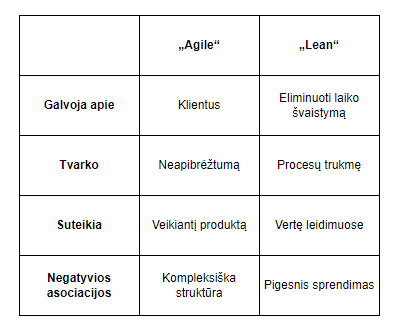
\includegraphics[scale=0.8]{img/AgileVSLean.png}
    \caption{„Agile“ ir „Lean“ metodų palyginimas}
    \label{img:mlp}
\end{figure}

\subsection{Išleidimų automatizacija}

Prieš tai aprašytos metodikos suteikia galimybes pagerinti leidimų pristatymo kokybę bei kokiu greičiu jie pasiekia produkcinę aplinką, bet tai virsta realybe tik tuo metu, jei viskas yra įgyvendinama idealiai, procesų eiga nekinta arba kinta neženkliai. Todėl norint išvengti žmogiškųjų klaidų, kurios gali lemti dideles nesėkmes išleidimo valdyme - autoriaus nuomone siekiamybė turėtų būti automatizuoti procesus, kurie tiksliai apibrėžtų įvykių seka bei veiksmus, kurie turėtų būti atlikti automatiškai. Tai sutaupo ne tik laiko resursus, kadangi reikalinga mažesnė priežiūra iš sistemos administratorių, bet ir sprendžia prieš tai aprašytą problemą, jog kiekvieną kartą įvykus tam pačiam scenarijui bus vykdomi tie patys aprašyti žingsniai ir nėra žmogiškojo faktoriaus.

    \subsubsection{„DevOps“ pozicijos svarba leidimų valdyme}

% TODO: Citatą į išnašas
Automobilių kompanijos „Ford“ įkūrėjas Henry Fordas yra pasakęs: „Jei aš būčiau paklausęs žmonių, ko jie nori, jie būtų atsakę – greitesnių arklių". Ši mintis galėtų būti pritaikyta klasikiniai sistemos administratoriaus pozicijai. Kadangi tinkamų įrankių automatizacijai trūkumas, žmogiškų klaidų didelis skaičius bei prasta komunikacija tarp komandų buvo sprendžiama ne su tos profesijos žmonėmis, nes buvo susiformavęs supratimas, jog tai sistemos administratorių pareiga automatizuoti programinės įrangos leidimus, testų patikras ir kitas reikalingas veiklas \cite{SaltTrecias}. Dėl šios priežasties ir atsirado pozicija - „DevOps“. Siekiant išspręsti išvardintas problemas „DevOps“ inžinierius visapusiškai siekia dalyvauti programinės įrangos kūrimo cikle bei spręsti komunikacijos problemas, kurios dažnai kyla tradiciniame leidimų valdyme. Tuomet šią poziciją užimantis asmuo ieško būdu automatizuoti kodo paruošimo, testavimo ir išleidimo veiklas derinant poreikius reikalingus tiek programuotojams, tiek sistemos administratoriams. Autoriaus nuomone tai leidžia sėkmingai atskirti programuotojų bei sistemos administratorių veiklas ir skirti didesnį dėmesį programinės įrangos išleidimo valdymui.

\begin{figure}[H]
    \centering
    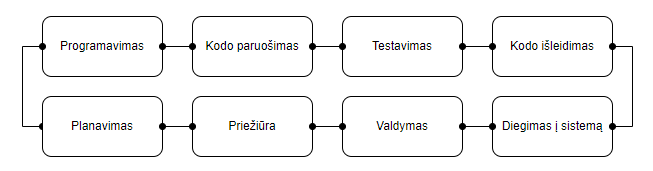
\includegraphics[scale=0.8]{img/DevOps.png}
    \caption{PĮ veiklos tarp kurių „DevOps“ inžinieriai siekia automatizuoti procesus}
    \label{img:mlp}
\end{figure}

    \subsubsection{Nepertraukiamas diegimas į aplinkas}
    
Nepertraukiamas diegimas (angl. \textit{Continuous Deployment}) yra programinės įrangos išleidimo strategija, kai kodo pakeitimai yra automatiškai sukompiliuojami, testuojami ir diegiami į produkcinę aplinką. Šis metodas gali sutrumpinti laiką, per kurį kodo pakeitimai (t.y. nauji leidimai) pasiekia vartotojus. Svarbiausias automatizacijos pranšumas yra klaidų rizikos sumažinimas, nes visi leidimai yra automatiškai tikrinami prieš įdiegiant juos. Paprastai šios metodikos įgyvendinimui yra paskirta prieš tai aptartų „DevOps“ inžinierių komanda. Norimiems rezultatams pasiekti reikalingi įvairūs automatizavimo įrankiai, testavimo sistemos, taip pat ir versijų valdymo sistemos (tokios kaip „Git“) įskaitant ir šakojimosi strategijas (angl. \textit{Branching strategies}), pagal kurias visi procesai ir bus ruošiami automatizacijai. Tačiau norint turėti automatinius ir nepertraukiamus diegimus į sistemą yra reikalingi reikšmingi pakitimai procesuose, net jei ir naudojamos įprastos praktikos tokios kaip „Agile“, nes ši metodika yra dar jauna ir yra atlikta nedaug empirinių tyrimų \cite{SaltSeptintas}. Tai kelia kėblumų įmonėms įsigyvendinti, nes nėra taip aiškiai apibrėžtų gairių kaip tos sistemos turėtų veikti, todėl yra reikalingi nemaži finansiniai bei laiko resursai, kad procesai būtų automatizuoti kiekvienam sprendimui individualiai. Taip pat yra reikalingi dar papildomi kaštai, kurie yra naudojami ne tik automatizuotų procesų kurimui, bet taip pat ir jų priežiūrai vėliau, nes programinė įranga yra dinamiškai kintantis dalykas, todėl ir procesų veikimas pagal situaciją turėtų kisti.
    
    \subsubsection{Skirtingos „Git“ šakojimosi strategijos leidimų valdyme}

Pagal atliktą „Stackoverflow“ tyrimą 2022 metais tarp visų versijavimo sistemų - „Git“ buvo paminėta beveik 94 procentų kartų \cite{SaltAstuntas}. Todėl „Git“ šakojimosi strategijos yra labai svarbi sudedamoji dalis PĮ išleidimų valdyme, leidžianti programuotojams turėti atskiras savo kodo šakas (angl. \textit{branch}), kurios suteikia galimybę dirbti su naujais funkcionalumais ar klaidų taisymais nerizikuojant pažeisti pagrindinės kodo bazės. Šiuo metu egzistuoja daug skirtingų strategijų, kurias organizacijos gali pritaikyti atsižvelgdamos į savo poreikius. Pasirinkta strategija daro labai didelę įtaką visam išleidimų valdymo procesui, nes įprastai šakos su pavadinimais „Production“, „Staging“ ar „Development“ turi programinį kodą, kurį automatizuoti procesai naudoja atitinkamoms aplinkoms pagal pavadinimą įdiegti.

        \subsubsubsection{„GitFlow“ metodas}

Šis šakojimosi strategijos metodas suteikia programuotojams galimybę dirbti su keliais funkcionalumais tuo pačiu metu sukuriant po atskirą šaką kiekvienam iš jų. Jos yra sukuriamos išvedant iš pagrindinės šakos (paprastai vadinamos „Development“ arba „Develop“). Kai darbas su specifiniu funkcionalumu yra pabaigtas (t.y. kodas yra parašytas, patestuotas bei patvirtintas kitų kolegų kaip tinkamas), pakeitimai yra įliejami į pagrindinę šaką. Tačiau „GitFlow“ turi ir daugiau kompleksiškumo - skirtingai nei kai kuriuose kituose metoduose, naujas programinis kodas produkcinės aplinkos iškart nepasiekia po kodo suliejimo į pagrindinę šaką. Norint turėti naują leidimą į produkcinę aplinką - kuriamos atskiros leidimų šakos su nurodyta versija, tai leidžia turėti paraleliai daug produkcinių aplinkų su skirtingomis versijomis. Bet svarbu pastebėti, kad tai labai pailgina visą nepertraukiamo diegimo į aplinkas procesą, todėl kai yra reikalingi greiti pataisymai yra kuriamos šakos, kurios yra atskiros nuo visos struktūros, kad jos tiesiai keliautų į produkcinės aplinkos šaką, o iš jos automatinių procesų pagalba leidimas pasiekia klientų naudojamą produktą. Šiai strategijai išpildyti yra kuriamos tokio tipo šakos:

\begin{itemize}
    % TODO: Suinteresuotos šalys - įdėti į sąvokas
  \item \textit{Production (Master)}. Šaka, kurioje laikomas visas produkcinės aplinkos kodas. Į ją kodas suliejamas tik iš tokių šakų kaip „Release“ ar „Hotfix“.
  
  \item \textit{Development (Develop)}. Ši šaka kaupia visą kodą, kuris yra produkcinėje aplinkoje, tik dar ir į ją yra suliejami nauji funkcionalumai iš „Feature“ tipo šakų. Kai norima naujo leidimo su įgyvendintu nauju kodu - iš šios šakos yra kuriama nauja, „Release“ tipo.

  \item \textit{Feature (feature-*)}. Kiekvienas naujas funkcionalumas turi savo atskirą šaką, kurioje yra kaupiamas visas kodas susijęs tik su tuo sprendimu. Galiausiai, kai kodas yra pilnai paruoštas, ši šaka yra liejama į „Development“ šaką.

  \item \textit{Hotfix (hotfix-*)}. Šio tipo šakos yra naudojamos tik ypatingais atvejais, kuomet yra reikalingi skubūs kodo klaidų ištaisymai susiję su produkcine aplinka. Jose parašytas programinis kodas suliejamas tiesiogiai su produkcinės aplinkos šaka.

  
  \item \textit{Release (release-*)}. Kai yra pasiruošiama naujam leidimui - kuriama šio tipo šaka. Paprastai savo pavadinime ji saugo versijos numerį. Jos pagrindinis tikslas yra būti pereinamąja dalimi tarp programuotojų aplinkos ir produkcinės aplinkos. Pagrindinis pranašumas naudoti šį tipą yra galimybė turėti paraleliai daug produkcinių aplinkų, sekti istoriją bei versijas.
\end{itemize}

Autoriaus nuomone didelis šio metodo kompleksiškumas gali sukurti ir nemažai problemų įmonėms, kurioms tokios stiprios kontrolės ir priežiūros nereikia. Imitavus vos poros funkcionalumų, vienos kritinės klaidos ir keletos paprastų klaidų scenarijų - kompleksiškumas išauga eksponentiškai.

\begin{figure}[H]
    \centering
    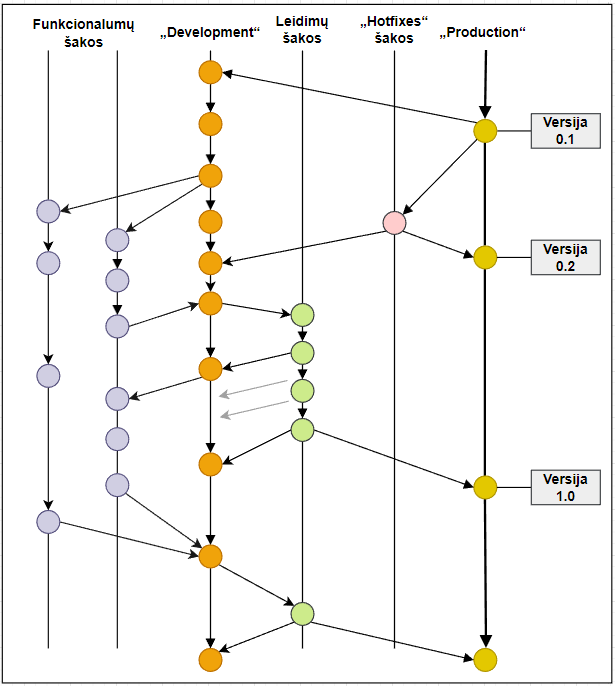
\includegraphics[scale=0.6]{img/GitFlowBold.png}
    \caption{„GitFlow“ metodo pavyzdinio scenarijaus iliustracija}
    \label{img:mlp}
\end{figure}

        \subsubsubsection{„GitHub Flow“ ir „GitLab Flow“ metodai}

Ši „Git“ šakojimosi strategija pasižymi paprastumu ir patogumu naudotis. Iš esmės ji veikia labai panašiu principu kaip ir jau aptartas „GitFlow“ metodas, tik yra atsisakoma tokių šakų tipų kaip: „Hotfix“, „Release“, „Development“. Dirbama tik su „Feature“ tipo šakomis, kuriose yra kuriami nauji funkcionalumai ir juos pabaigus bei komandos nariams užtvirtinus, kad nauja kodo bazė paruošta tinkamai - ji yra suliejimas į šaką „Production“. Ji visada yra palaikoma nepertraukiamo diegimo ir vos tik funkcionalumas pasiekia produkcinės aplinkos šaką - automatizuoti procesai įdiegia į klientų naudojamą programą naują leidimą \cite{SaltDevintas}. Tačiau sumažintas kompleksiškumas sukuria nemažai ir problemų - lyginant su pirmuoju metodu nebėra saugoma istorija versijų, produkcinis kodas gali būti nestabilus, nes nėra tarpinės šakos tarp funkcionalumo ir „Production“ šakų.

Tuo tarpu „GitLab Flow“ irgi yra paprastesnė „GitFlow“ alternatyva, tik skirtingai nuo „GitHub“ sukurto sprendimo, šis vietoj vienos produkcinės aplinkos šakos, turi dvi pagrindines \cite{SaltDesimtas}:

\begin{itemize}
    % TODO: Suinteresuotos šalys - įdėti į sąvokas
  \item \textit{Staging}. Šaka į kurią yra suliejamos naujų funkcionalumų ar klaidų taisymo šakos. Joje esantis kodas automatinių procesų pagalba visada yra atnaujinimas su kiekvienu suliejimu ir įdiegiamas į stabilią, bet ne produkcinę aplinką (ji paprastai yra pasiekiama tik užsakovams, programuotojams ir produktą integruojančioms kitoms įmonėms).
  
  \item \textit{Production}. Kai nusprendžiama, kad stabilioje aplinkoje esantis kodas yra tinkamas - jis suliejamas iš „Staging“ šakos į šią. Tuomet lygiai taip pat - automatiniai procesai užtikrina, jog naujas diegimas pasiektų produkcinę aplinką, kuria jau naudojasi patys vartotojai.

\end{itemize}

% TODO: Parašyti papildomą sakinį apie palyginimą su GitFlow, kad žymiai paprasčiau ir t.t., tada padaryti irgi pavyzdinio scenarijaus schemą, kuri parodytų, kad čia jau viskas veikia žymiai paprasčiau

        \subsubsubsection{„Trunk-based development“ metodas}

Šios strategijos pagrindinis skirtumas yra tas, kad programuotojai dirba tiesiogiai su pagrindine šaka, dar kitaip vadinama šiame metode - kamienu (angl. \textit{trunk}). „Trunk-based development“ siekia, kad kodas visada būtų stabilus ir pasiruošęs diegimui ir programuotojai galėtų greit bei efektyviai įgyvendinti mažus pakitimus be jokių papildomų trikdžių. Tai yra įmanoma, kadangi nėra naudojamos jokios kitos papildomos šakos, o funkcionalumai atskiriami žymėmis (angl. \textit{tags}), kurios apibrėžia kokį kodą programutojas paruošė. Autoriaus nuomone, tai yra viena rizikingiausių strategijų, nes kodas nėra tinkamai peržiūrimas ir keliauja tiesiai į produkcinę aplinką, tačiau programinės įrangos išleidimo valdymas yra primityvus, net ir tuomet, kai kuriama daug funkcionalumų.

\begin{figure}[H]
    \centering
    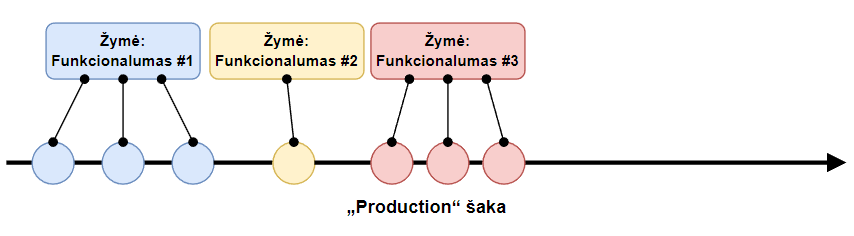
\includegraphics[scale=0.6]{img/TrunkBased.png}
    \caption{„Trunk-based development“ metodo pavyzdinio scenarijaus iliustracija}
    \label{img:mlp}
\end{figure}

% is a branching strategy where developers work directly on the main branch, also known as the "trunk." This means that there is only one main branch, and all code changes are made directly to it. This strategy is based on the idea that the trunk should always be in a stable and deployable state, and that developers should be able to make small, frequent changes to the codebase without causing disruptions.

% yra šakojimo strategija, kai kūrėjai dirba tiesiogiai su pagrindine šaka, dar vadinama „kamienu“. Tai reiškia, kad yra tik viena pagrindinė šaka, o visi kodo pakeitimai atliekami tiesiai į jį. Ši strategija pagrįsta idėja, kad bagažinė visada turi būti stabilios ir įdiegiamos būsenos, o kūrėjai turėtų turėti galimybę atlikti nedidelius, dažnus kodų bazės pakeitimus, nesukeldami trikdžių.

% Straipsniai
% https://www.flagship.io/git-branching-strategies/
% https://medium.com/@patrickporto/4-branching-workflows-for-git-30d0aaee7bf

% 2 dalis. Laikinosios aplinkos
\section{Laikinųjų aplinkų strategijos analizė}
Medžiagos darbo tema dėstymo skyriuose pateikiamos nagrinėjamos temos detalės:
pradinė medžiaga, jos analizės ir apdorojimo metodai, sprendimų įgyvendinimas,
gautų rezultatų apibendrinimas. Šios dalies turinys labai priklauso nuo darbo
temos. Skyriai gali turėti poskyrius ir smulkesnes sudėtines dalis, kaip
punktus ir papunkčius.

Medžiaga turi būti dėstoma aiškiai, pateikiant argumentus. Tekstas dėstomas
trečiuoju asmeniu, t.y. rašoma ne „aš manau“, bet „autorius mano“, „autoriaus
nuomone“. Reikėtų vengti informacijos nesuteikiančių frazių, pvz., „...kaip jau
buvo minėta...“, „...kaip visiems žinoma...“ ir pan., vengti grožinės literatūros
ar publicistinio stiliaus, gausių metaforų ar panašių meninės išraiškos
priemonių.

\subsection{Poskyris}
Citavimo pavyzdžiai: cituojamas vienas šaltinis

\subsubsection{Skirsnis}
\subsubsubsection{Straipsnis}
\subsubsection{Skirsnis}


%  3 dalis. Praktinė dalis
\section{Praktinis laikinųjų aplinkų sprendimas}
\subsection{Poskyris}
\subsection{Poskyris}

\sectionnonum{Rezultatai ir išvados}
Rezultatų ir išvadų dalyje turi būti aiškiai išdėstomi pagrindiniai darbo
rezultatai (kažkas išanalizuota, kažkas sukurta, kažkas įdiegta) ir pateikiamos
išvados (daromi nagrinėtų problemų sprendimo metodų palyginimai, teikiamos
rekomendacijos, akcentuojamos naujovės).

% TODO: Peržiūrėti, kad nebūtų piratuotų straipsnių link'ų
\printbibliography[heading=bibintoc]  % Šaltinių sąraše nurodoma panaudota
% literatūra, kitokie šaltiniai. Abėcėlės tvarka išdėstomi darbe panaudotų
% (cituotų, perfrazuotų ar bent paminėtų) mokslo leidinių, kitokių publikacijų
% bibliografiniai aprašai.  Šaltinių sąrašas spausdinamas iš naujo puslapio.
% Aprašai pateikiami netransliteruoti. Šaltinių sąraše negali būti tokių
% šaltinių, kurie nebuvo paminėti tekste.

% \sectionnonum{Sąvokų apibrėžimai}
\sectionnonum{Santrumpos}
Sąvokų apibrėžimai ir santrumpų sąrašas sudaromas tada, kai darbo tekste
vartojami specialūs paaiškinimo reikalaujantys terminai ir rečiau sutinkamos
santrumpos.

\appendix  % Priedai
% Prieduose gali būti pateikiama pagalbinė, ypač darbo autoriaus savarankiškai
% parengta, medžiaga. Savarankiški priedai gali būti pateikiami ir
% kompaktiniame diske. Priedai taip pat numeruojami ir vadinami. Darbo tekstas
% su priedais susiejamas nuorodomis.

\section{Neuroninio tinklo struktūra}
\begin{figure}[H]
    \centering
    \includegraphics[scale=0.5]{img/MLP}
    \caption{Paveikslėlio pavyzdys}
    \label{img:mlp}
\end{figure}


\section{Eksperimentinio palyginimo rezultatai}
% tablesgenerator.com - converts calculators (e.g. excel) tables to LaTeX
\begin{table}[H]\footnotesize
  \centering
  \caption{Lentelės pavyzdys}
  {\begin{tabular}{|l|c|c|} \hline
    Algoritmas & $\bar{x}$ & $\sigma^{2}$ \\
    \hline
    Algoritmas A  & 1.6335    & 0.5584       \\
    Algoritmas B  & 1.7395    & 0.5647       \\
    \hline
  \end{tabular}}
  \label{tab:table example}
\end{table}

\end{document}
